
\section{Introduction}
\label{sec:intro}
% Backgound
\begin{figure}
    \centering
    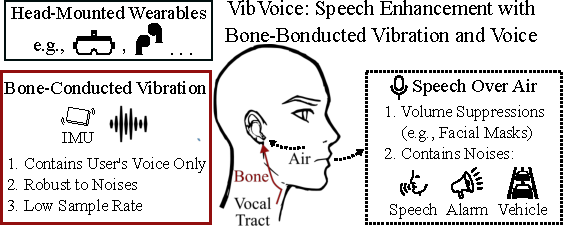
\includegraphics[width=\columnwidth]{chapters/vibvoice/figure/intro.pdf}
        %\vspace{-1em}
    \caption{VibVoice enhances speech quality of head-mounted wearables by extracting the user's clear voice from the bone-conducted vibrations.}
    \label{fig:intro}
\end{figure}
Head-mounted wearables, or HMWs, are smart devices that can be put on users' heads or ears, which include True Wireless Stereo (TWS) earphones, VR/AR headsets, and smart glasses. HMWs are equipped with several sensors and run various applications like VR/AR, motion recognition, and voice assistants. Represented by TWS earphones like the Apple Airpods series, the shipment of HMWs has grown as the largest category among all wearable devices, estimated to be more than $273$ million units worldwide in 2023 \citep{wearable-stat}. 
Manufacturers are adding various functions to HMWs. For example, some HMWs (especially earphones and headphones) support active noise cancellation (ANC) to improve the listening experience. On the speech side, voice-related applications using HMW s microphones are among the most frequently used. 

For example, an increasing number of people make phone calls with TWS earphones.
Through voice commands, users can also interact with voice assistants (e.g., Siri and Alexa). 
However, the speech quality on HMWs is unsatisfactory due to the following challenges:
First, most HMWs adopt omnidirectional microphones that can receive audio from any angle, leading to extra environmental noises.
Second, although most HMWs are equipped with multiple microphones to form an array and remove noises based on beamforming, the microphones on HMWs are too close to achieving a satisfying performance. 
Third, the speech audio is significantly suppressed when it reaches the HMWs as the HMWs are usually far away from the user's mouth.
Lastly, the worldwide pandemic forces people to wear masks, which can further reduce the audio intensity.

% Existing approach
Various approaches have been developed for speech enhancement. Signal processing-based methods \citep{ephraim1995signal} remove noises based on their statistical models. However, these approaches cannot handle complex environments. Microphone beamforming \citep{yousefian2014hybrid,ji2017coherence} removes noises based on their directions. But they fail to distinguish the speaker's voice and noise when the microphones are placed too close. Several research \citep{subakan2021attention, zhang2021microphone, chatterjee2022clearbuds} adopt deep neural networks (DNNs) to improve speech quality. However, their performance varies when the domain changes.  
Except for the audio-only solution, several works leverage other modalities like contact sensors \citep{gupta2018precision}, vibration sensor \citep{maruri2018v}, camera \citep{ gao2021visualvoice}, mm-Wave Radar \citep{ozturk2021radiomic, li2020vocalprint, liu2021wavoice}, ultrasonic sensing \citep{sun2021ultrase, zhang2021sensing}, and Lidar \citep{sami2020spying}, which introduce additional hardware requirements or user overhead to existing HMWs.

% Technical Challenges
Inertial Measurement Unit (IMU) is a common sensor on most HMWs and can capture audio with a direct connection with the speaker \citep{ba2020learning, wang2021audio}. Since HMWs are well connected to the user's head, the IMU accelerometer can sense the vibrations caused by the speaker's voice through the skull's bone conduction. The bone-conducted vibration contains speech from the user only without environmental noises or voices. However, the accelerometer on HMWs has a low sample rate (e.g., $1.6~\text{kHz}$) due to the limited size and energy consumption, which is not enough to recover the human's voice (e.g., up to $3.4~\text{kHz}$ \citep{Voicefre75:online}). 

We propose \textit{VibVoice}, the first end-to-end multi-modal speech enhancement system for HMWs using the bone conduction from the vibration to the audio. The design of VibVoice fits mobile devices, considering the on-device sensor, execution latency, and communication overhead.
VibVoice exploits the complementary characteristics of the two modalities: the acceleration has a low sample rate covering a partial audible spectrum but with no environmental noises. The microphone has a high sample rate covering the whole audible spectrum but is mixed with ambient voice and noises. Such a combination of modalities provides a stable reference for extracting the target speech.
VibVoice uses a DNN to reconstruct clean speech with two encoders and decoders for processing the data from two modalities, respectively. VibVoice faces three major technical challenges as follows:

\noindent\textbf{Lack of paired labeled acceleration and audio.}
Collecting a paired multi-modal dataset is labor-intensive. Although there are public datasets of either acceleration or audio, none has the paired data on head-mounted wearables. 
Collecting such a paired dataset on a large scale can introduce excessive overheads, such as recruiting diverse volunteers and recording hundreds of hours of audio with annotations. 

\noindent\textbf{Fusion of data with different modalities and sample rates.}
Microphone audio has much richer information than acceleration data due to the higher sample rate. As a result, the DNN is prone to overfitting and may ignore the data input of acceleration. 
Therefore, during the training of DNN, we require a special training strategy to avoid overfitting and two dedicated losses to balance the weights of the two modalities.

\noindent\textbf{Practical concern for deployment.} 
Deploying deep learning speech enhancement in the real world is non-trivial due to the variance among people's voice and bone conduction channels.    
Even though some users may tolerate a rapid data collection phase before use, the amount and quality of the collected data are not guaranteed for training a high-performance model.

To overcome the above challenges, we design VibVoice based on our extensive measurements of the bone-conduction effects on real-world data. We conclude our contributions as follows:
\begin{itemize}
    \item  We propose a novel estimation approach to model Bone Conduction Function with a limited dataset to augment paired acceleration and audio based on a large public audio dataset. The augmented paired dataset can be used for model training. 
    \item We design a two-branch DNN that a) recovers the speech-related information from the acceleration signal with a low sample rate, b) extracts the clean speech from contaminated audio with the help of the acceleration signal, and c) has a lightweight design and can be run on the mobile device with low latency.
    \item We collect a two-modal dataset and evaluate VibVoice on a self-designed platform, \emph{EarSense}, equipped with an accelerometer and a microphone to acquire paired acceleration and audio data simultaneously. The dataset and the design of data collector are open-sourced.
\end{itemize}

We evaluate VibVoice on a paired acceleration and microphone from 15 volunteers. We test VibVoice's performance on the offline synthetic noise dataset and the concurrent noise dataset in various scenarios.
VibVoice achieves the best performance with 31 times less latency on mobile devices than the two strong baselines. In addition, data augmentation can reduce the requirement of paired data by more than 72 times.
We recruit 35 volunteers for a user study in which VibVoice is preferred by 87$\%$ users compared to the baseline.





